\section[Rentgenofluorescenční analýza]{Energiově a vlnově dispersní rentgenfluorescenční analýza}

\subsection{Princip metody}

Nedestruktivní metoda zjišťování chemického (prvkového) složení zkoumané látky.

Je založena na detekci charakteristického RTG záření, jež je emitováno příslušnými atomy prvků obsažených ve zkoumané látce. Nejprve je látka vystavěna dopadajícím fotonům (RTG záření například z rentgenky nebo gama z vhodného radionuklidu). Tyto fotony pak vyráží elektrony (nejčastěji z vnitřní slupky K, popř. L). Poté dochází k přeskoku elektronů z vyšší slupky na toto prázdné místo a rozdíl energií je vyzářen v podobě fluorescenčních fotonů RTG záření, které je specifické pro daný prvek.

\textbf{Kvalitativní analýza}: je možné díky detekci charakteristického RTG záření, jež je specifické pro daný prvek (detekujeme energii a vlnovou délku).

\textbf{Kvantitativní analýza}: množství emitovaných fotonů charakteristického záření je přímo úměrné množství atomů daného druhu a je tedy mírou koncentrace daného prvku. Kvantita je dána intenzitou jednotlivých píků fluoroscenčního záření.

Vlnová délka charakteristického RTG záření je klesající s rostoucím Z číslem prvků a naopak energie se zvyšuje se $Z$ číslem. Metoda RFA/XRF je dobrá pro prvky s větším $Z$, jelikož se lépe detekují.

\textbf{Výhody:} \begin{itemize}
    \item Rychlost, přesnost a reprodukovatelnost
    \item Vzorky mohou být v jakémkoliv skupenství
    \item Nedestruktivní metoda
    \item Multiprvková analýza
    \item Dobré pro zkoumání složení uměleckých předmětů
\end{itemize}

\textbf{Nevýhody:} \begin{itemize}
    \item Obtížná detekce prvků lehčích než $Z<13$
    \item Nerozpozná chemické sloučeniny
    \item Omezení na pouhý povrch zkoumaného materiálu
\end{itemize}

\begin{figure}[H]
    \centering
    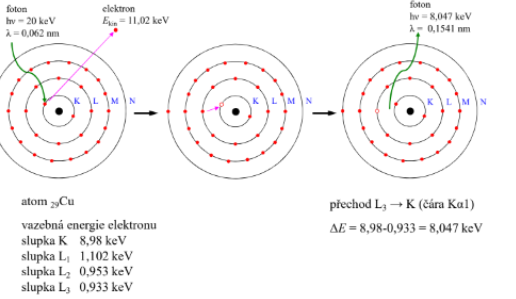
\includegraphics[width=0.9\linewidth]{img/Princip RFA 1.png}
    \caption{Princip RFA 1}
\end{figure}

\begin{figure}[H]
    \centering
    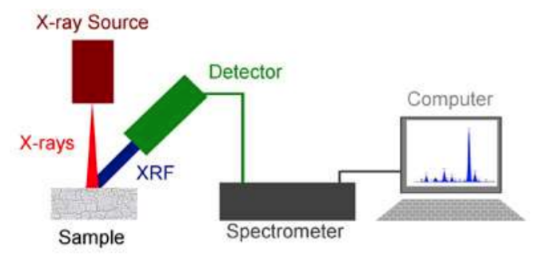
\includegraphics[width=0.7\linewidth]{img/Princip RFA 2.png}
    \caption{Princip RFA 2}
\end{figure}

\subsection{Vlnově disperzní RFA}

Ze skundárního charakteristikcého záření se izolují jednotlivé vlnové délky (čáry) spektra přes difrakci na krystalu. Poté je možné měřit intenzitu jednotlivých čar pro jednotlivé prvky postupně. Pokud máme multikrystal (složen z různých vrstev), pak je možné provádět analýzu současně.

Používá se při kvantitativní analýze prvků B po U (materiál v podobě pevné, zrnité i kapalné)

Vyžaduje velké rozměry přístrojů, vysokou spotřebu energie, ale dosahuje velmi dobrých technických parametrů.

Sekundární záření se odráží na krystalu a dopadá do detektoru/čítače (difrakce je dána Braggovým zákonem).

V závislosti na $Z$ prvků, které chci měřit, tak se volí krystaly:

\begin{itemize}
    \item Pro těžké a středně těžké prvky (= krátké vlnové délky) je používají LiF, NaCl, Ge, InSb.
    \item Pro lehčí prvky se využívají soli organických kyselin s těžkým kovem (ten tvoří uzlové body v krystalové mřížce).
    \item Pro velmi lehké prvky se používají uměle připravené multivrstevnaté krystaly (kde se do matrice lehkého prvku (Si) vkládají vrstvy těžkého kovu).
\end{itemize}

Výsledné spektrum je pak funkcí intenzity na vlnové délce či na difrakčním úhlu $2 \Theta$.

\begin{figure}[H]
    \centering
    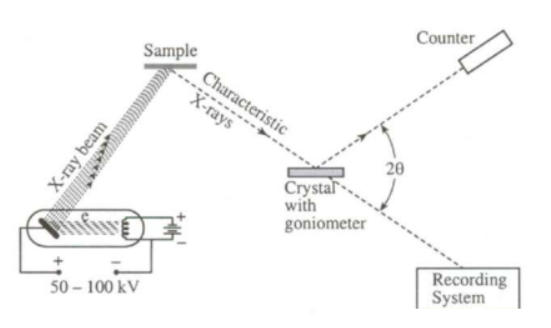
\includegraphics[width=0.8\linewidth]{img/Vlnově_disperzní_RFA.png}
    \caption{Vlnově disperzní RFA}
\end{figure}

\subsection{Energiově disperzní RFA}

Jedná se o menší a levnější přístroje, kde je analyzováno celé spektrum pomocí polovodičového detektoru (detekovaná energie je úměrná elektrickému impulzu a počet signálů o dané energii je roven intenzitě záření. Amplituda impulzů je úměrná energii).

Obvykle se využívá Si(Li) detektor, kde jsou vznikající impulsy zesíleny a tříděny dle velikosti pomocí MCA (četnost impulzů v kanálech = intenzita fotonů = kvantita).

Jsou zde horší detekční limity pro lehké prvky, takže spíše detekce prvků od Na po U (obecně nelze použít pro $Z<13$).

\subsection{Požadavky na vzorek pro RFA analýzu}

\begin{itemize}
    \item Pokud je vzorek v tuhé formě, měl by být ideálně zcela hladký a vyleštěný, aby se tam nepletla např. koroze a jiné blbosti (prach, apod..) $\rightarrow$ V zásadě jako metalografický výbrus.
    \item Zrnitý materiál se namele, aby byla zajištěna stejná distribuce částic a pak se lisuje do matrice/tablet.
    \item Kapalné vzorky jsou v pohodě.
    \item Aerosoly se taky dají, například pomocí záchytu na filtru, které se pak měří.
    \item Kapalné a práškové vzorky se měří za přítomnosti He.
    \item Stanovení lehkých prvků jde za přítomnosti vakua, protože lehké prvky mají sekundární záření o malé energii, takže se těžko detekují.
\end{itemize}

\subsection{Detektory pro RFA}

\textbf{Scintilační:} Monokrystal NaI(Tl), KI(Tl) + fotonásobič (základní měření)

\textbf{Polovodičové:} čisté Si nebo Ge dopovaného Li (přesnější měření, nejčastěji využívané):

\begin{itemize}
    \item Nejčastějji Si(Li) chlazené dusíkem.
    \item RTG foton vyvolá vznik páru elektron-díra a počet párů je pak úměrný energii fotonu. Hlavní výhodou je vysoké energetické rozlišení.
    \item Vysoké rozlišení, využívá MCA.
    \item Si(Li) -- mají větší detekční plochu a vyšší energetické rozlišení.
    \item SiPIN (Silicon pin diode detectors) -- pracují blízko pokojové teploty a stačí chlazení Peltierovým článkem, menší detekční plocha a srovnatelné energetické rozlišení (stále se vyvíjejí, využití v průzkumu kosmu), horší detekční účinnost.
    \item Laboratorní XRF -- obvykle ve vakuu, používají se však i mobilní XRF analyzátory (viz exkurze KDAIZ) $\rightarrow$ žádná příprava vzorku, měření na vzduchu, na různých místech, velmi rychlé. Ve formě pistolky, která obsahuje zdroj (rentgenku) a zároveň detektor.
\end{itemize}

\textbf{Plynové ionizační detektory:} už se spíše nevyužívají, mají horší rozlišení:

\begin{itemize}
    \item Např. proporciální detektory
    \item Průtokový či uzavřený detektor naplněný Ar, W anoda $\rightarrow$ měří se ionizační proud.
\end{itemize}